% Options for packages loaded elsewhere
\PassOptionsToPackage{unicode}{hyperref}
\PassOptionsToPackage{hyphens}{url}
%
\documentclass[
  12pt,
]{article}
\usepackage{lmodern}
\usepackage{amssymb,amsmath}
\usepackage{ifxetex,ifluatex}
\ifnum 0\ifxetex 1\fi\ifluatex 1\fi=0 % if pdftex
  \usepackage[T1]{fontenc}
  \usepackage[utf8]{inputenc}
  \usepackage{textcomp} % provide euro and other symbols
\else % if luatex or xetex
  \usepackage{unicode-math}
  \defaultfontfeatures{Scale=MatchLowercase}
  \defaultfontfeatures[\rmfamily]{Ligatures=TeX,Scale=1}
\fi
% Use upquote if available, for straight quotes in verbatim environments
\IfFileExists{upquote.sty}{\usepackage{upquote}}{}
\IfFileExists{microtype.sty}{% use microtype if available
  \usepackage[]{microtype}
  \UseMicrotypeSet[protrusion]{basicmath} % disable protrusion for tt fonts
}{}
\makeatletter
\@ifundefined{KOMAClassName}{% if non-KOMA class
  \IfFileExists{parskip.sty}{%
    \usepackage{parskip}
  }{% else
    \setlength{\parindent}{0pt}
    \setlength{\parskip}{6pt plus 2pt minus 1pt}}
}{% if KOMA class
  \KOMAoptions{parskip=half}}
\makeatother
\usepackage{xcolor}
\IfFileExists{xurl.sty}{\usepackage{xurl}}{} % add URL line breaks if available
\IfFileExists{bookmark.sty}{\usepackage{bookmark}}{\usepackage{hyperref}}
\hypersetup{
  pdftitle={Black Lives Matter Protests and Voter Turnout},
  pdfauthor={Cameron Kimble; Kevin Morris; Kasey Zapatka},
  hidelinks,
  pdfcreator={LaTeX via pandoc}}
\urlstyle{same} % disable monospaced font for URLs
\usepackage[margin=1in]{geometry}
\usepackage{longtable,booktabs}
% Correct order of tables after \paragraph or \subparagraph
\usepackage{etoolbox}
\makeatletter
\patchcmd\longtable{\par}{\if@noskipsec\mbox{}\fi\par}{}{}
\makeatother
% Allow footnotes in longtable head/foot
\IfFileExists{footnotehyper.sty}{\usepackage{footnotehyper}}{\usepackage{footnote}}
\makesavenoteenv{longtable}
\usepackage{graphicx}
\makeatletter
\def\maxwidth{\ifdim\Gin@nat@width>\linewidth\linewidth\else\Gin@nat@width\fi}
\def\maxheight{\ifdim\Gin@nat@height>\textheight\textheight\else\Gin@nat@height\fi}
\makeatother
% Scale images if necessary, so that they will not overflow the page
% margins by default, and it is still possible to overwrite the defaults
% using explicit options in \includegraphics[width, height, ...]{}
\setkeys{Gin}{width=\maxwidth,height=\maxheight,keepaspectratio}
% Set default figure placement to htbp
\makeatletter
\def\fps@figure{htbp}
\makeatother
\setlength{\emergencystretch}{3em} % prevent overfull lines
\providecommand{\tightlist}{%
  \setlength{\itemsep}{0pt}\setlength{\parskip}{0pt}}
\setcounter{secnumdepth}{5}
\usepackage{rotating}
\usepackage{setspace}
\usepackage{booktabs}
\usepackage{longtable}
\usepackage{array}
\usepackage{multirow}
\usepackage{wrapfig}
\usepackage{float}
\usepackage{colortbl}
\usepackage{pdflscape}
\usepackage{tabu}
\usepackage{threeparttable}
\usepackage{threeparttablex}
\usepackage[normalem]{ulem}
\usepackage{makecell}
\usepackage{xcolor}
\newlength{\cslhangindent}
\setlength{\cslhangindent}{1.5em}
\newenvironment{cslreferences}%
  {\setlength{\parindent}{0pt}%
  \everypar{\setlength{\hangindent}{\cslhangindent}}\ignorespaces}%
  {\par}

\title{Black Lives Matter Protests and Voter Turnout\thanks{The authors thank XX for their feedback and support. All errors are our responsibility.}}
\author{Cameron Kimble\footnote{Research and Program Associate, Brennan Center for Justice (\href{mailto:cameron.kimble@nyu.edu}{\nolinkurl{cameron.kimble@nyu.edu}})} \and Kevin Morris\footnote{Researcher, Brennan Center for Justice (\href{mailto:kevin.morris@nyu.edu}{\nolinkurl{kevin.morris@nyu.edu}})} \and Kasey Zapatka\footnote{PhD Student, CUNY Graduate Center (\href{mailto:kzapatka@gradcenter.cuny.edu}{\nolinkurl{kzapatka@gradcenter.cuny.edu}})}}
\date{February 02, 2021}

\begin{document}
\maketitle
\begin{abstract}
In the summer of 2020, Americans took to the streets in larger numbers than ever before. Following the police murders of George Floyd and Breonna Taylor, an enormous multiracial coalition voiced their dissatisfaction with the state of policing in the United States. These mass protests took place shortly before a presidential election, and the incumbent loudly voiced his disdain for protesters and their political message. This paper explores one aspect of the impact of the Black Lives Matter (BLM) movement. Using a national voter file and data on protest location, we aim to estimate the causal impact of physical proximity to a BLM protest on voter turnout. Our pilot studies using Georgia, North Carolina, and Ohio point to a complicated relationship that demands further investigation.
\end{abstract}

\pagenumbering{gobble}
\pagebreak

\pagenumbering{arabic}
\begin{center}
Black Lives Matter Protests and Voter Turnout

Cameron Kimble, Kevin Morris, and Kasey Zapatka
\end{center}

Political socialization --- that is, the gradual development of an individual's political preferences, their perceptions of the political world and the state, and the internalization of their society's norms and behaviors (Fillieule \protect\hyperlink{ref-Fillieule2013}{2013}) --- has received increasing attention in recent years. Research about how individuals develop identities as citizens and engage in political behavior is being studied with increasing sophistication by sociologists and political scientists alike. Understanding when residents re-examine the legitimacy of the state and their relationship to it is of great importance to both scholars and activists, as is an examination of the political consequences. This paper furthers our understanding of how these processes play out by examining whether exposure to Black Lives Matter (BLM) protests in the summer of 2020 increased voter turnout.

Our paper tests one aspect of the emancipatory power of the BLM movement and measures the effect these protests had on voter turnout. If protest exposure led to increased voter turnout, it could provide evidence that BLM issues were salient in the minds of voters and represented an important mobilizing issue that should be considered in future elections. Specifically, we plan to use spatial regression techniques to test if distance from a BLM protest in June 2020 led to increased voter turnout in November.

\hypertarget{theory-and-literature}{%
\subsubsection*{Theory and Literature}\label{theory-and-literature}}
\addcontentsline{toc}{subsubsection}{Theory and Literature}

Foundational research on political socialization indicates that that initial \emph{frame alignment} (or a ``schemata of interpretation'') between an individual and a social movement or organization is a precondition for participation (Snow et al. \protect\hyperlink{ref-Snow1986}{1986}). That frame alignment is a continuous process that occurs between individuals and social movements, transforming and reinforcing the individual's ideological orientations. By their very nature, protest movements offer the opportunity for a frame realignment. By encouraging residents to reexamine the legitimacy of the police and state, the Black Lives Matter protests offered the possibility of just this sort of frame realignment.

There is, however, remarkably little literature on the political effects of mass protest in the United States. One study found that participating in the Freedom Summer project ``radicalized''volunteers, who were then significantly more likely to participate in social movements in subsequent years (McAdam \protect\hyperlink{ref-McAdam1989}{1989}). In a similar study, researchers conclude that involvement with social movements through the 1960s and 1970s caused a liberal shift in political orientation, as evidenced by subsequent political engagement such as voting for Jimmy Carter and participating in subsequent demonstrations (Sherkat and Blocker \protect\hyperlink{ref-Sherkat1997}{1997}).

Other scholars have documented the process by which cultural grievance is used to mobilize groups of voters in the post-New Deal United States (Leege et al. \protect\hyperlink{ref-Leege2002}{2002}). When social movements challenge the status quo, mobilization efforts from the associated political party intensifies, thereby increasing voter turnout (Winders \protect\hyperlink{ref-Winders1999}{1999}).

\hypertarget{the-mobilizing-potential-of-injustice-narratives}{%
\subsubsection*{The Mobilizing Potential of Injustice Narratives}\label{the-mobilizing-potential-of-injustice-narratives}}
\addcontentsline{toc}{subsubsection}{The Mobilizing Potential of Injustice Narratives}

Although protests can be a key site of political socialization, the Black Lives Matter movement centers on a social issue that has historically been \emph{demobilizing.} Indeed, a whole body of research has documented the legal estrangement (Bell \protect\hyperlink{ref-Bell2017}{2017}) that grows at the intersection of structurally unjust policies and a ``cultural orientation'' that views the criminal legal system as illegitimate and irrelevant (Kirk and Papachristos \protect\hyperlink{ref-Kirk2011}{2011}). This has led to institutional avoidance of many sorts (see Brayne \protect\hyperlink{ref-Brayne2014}{2014}), especially when it comes to voter participation (Lerman and Weaver \protect\hyperlink{ref-Lerman2014}{2014}). These demobilizing effects may extend even to individuals who have \emph{not} been formally convicted, but rather are in close contact with those who have been (Morris \protect\hyperlink{ref-Morris2020}{2020}; but see White \protect\hyperlink{ref-White2019}{2019}). The relationship, however, is complicated: Walker (\protect\hyperlink{ref-Walker2014}{2014}) shows that individuals in ``proximal contact'' with individuals who have been convicted become more likely to participate in non-electoral political activities such as attending a protest or donating money to a campaign.

Walker (\protect\hyperlink{ref-Walker2020}{2020}), however, provides key insight into how the demobilizing effects of contact with the legal system can be a \emph{mobilizing} force. Walker argues that, when individuals locate their experience with the legal system in narratives of (racial) injustice, the contact can spur them to take action. The Black Lives Matter movement has aimed to do just this. BLM activists have called attention to the fact that US police forces have a long history of racially discriminatory practices. The widespread protests may have caused individuals in close contact with police and the legal system to understand their contact with the police and legal systems \emph{not} as personal failings but as a result of racial inequity, which Walker's recent work indicates can catalyze turnout.

\hypertarget{data-and-methods}{%
\subsubsection*{Data and Methods}\label{data-and-methods}}
\addcontentsline{toc}{subsubsection}{Data and Methods}

To understand the relationship between protests and turnout, we leverage two primary datasets. First, we employ geocoded data from the US Crisis Monitor\footnote{See \url{https://acleddata.com/download/22846/}.} that records the location of every Black Lives Matter protest during 2020..

Our second data source is the national, geocoded voter file made available by L2 Political. The voter file includes a host of information about every registered voter in the country, including their gender, age, partisan affiliation, and race (L2 imputes the characteristics that are not reported in each state's public voter file). The registered voter file also includes information on voter turnout for the 2020 and previous elections. However, as of writing, not all states have yet entered their 2020 voter turnout into the registered voter file.

We intend to measure whether how far a voter lived from a Black Lives Matter protest in the summer of 2020 was correlated with their turnout in November. We measure the distance between each voter and the closest protest using geocoded records and test whether this distance is significantly related to turnout after controlling for other relevant characteristics, \emph{including} past turnout.

To be sure, this cannot prove the causal link between exposure to protest and increased turnout. Voters were not ``randomly'' exposed to protests; the same factors that primed an area to stage a protest may have also primed them to turn out at higher rates in the 2020 election. To identify the causal effect of exposure to protest on voter turnout we will leverage variation in rainfall (relative to historical rainfall) in the week following the murder of George Floyd as an instrument for protest exposure. Following established literature, we expect that rainfall in early June was correlated with protest formation, but not related (via mechanisms other than protest formation) to turnout in November. For a fuller discussion of how rainfall can be used to instrument political protests, see Madestam et al. (\protect\hyperlink{ref-Madestam2013}{2013}).

\hypertarget{preliminary-results}{%
\subsubsection*{Preliminary Results}\label{preliminary-results}}
\addcontentsline{toc}{subsubsection}{Preliminary Results}

As mentioned above, individual-level turnout records are not yet widely available, but will be published in the first half of 2021. However, records are available for Georgia, North Carolina, and Ohio, which we use as pilot studies.

Figure \ref{fig:map} reports the location of all protests staged in June, 2020, in our three pilot states.

\begin{figure}[H]
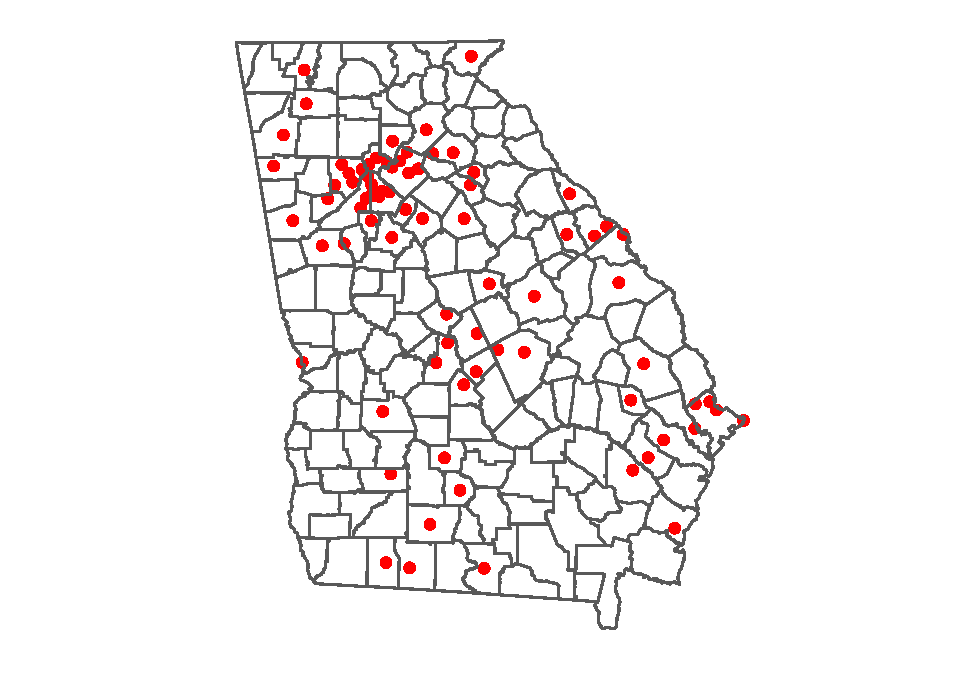
\includegraphics[width=0.32\linewidth]{asa_abstract_files/figure-latex/figures-side-1} 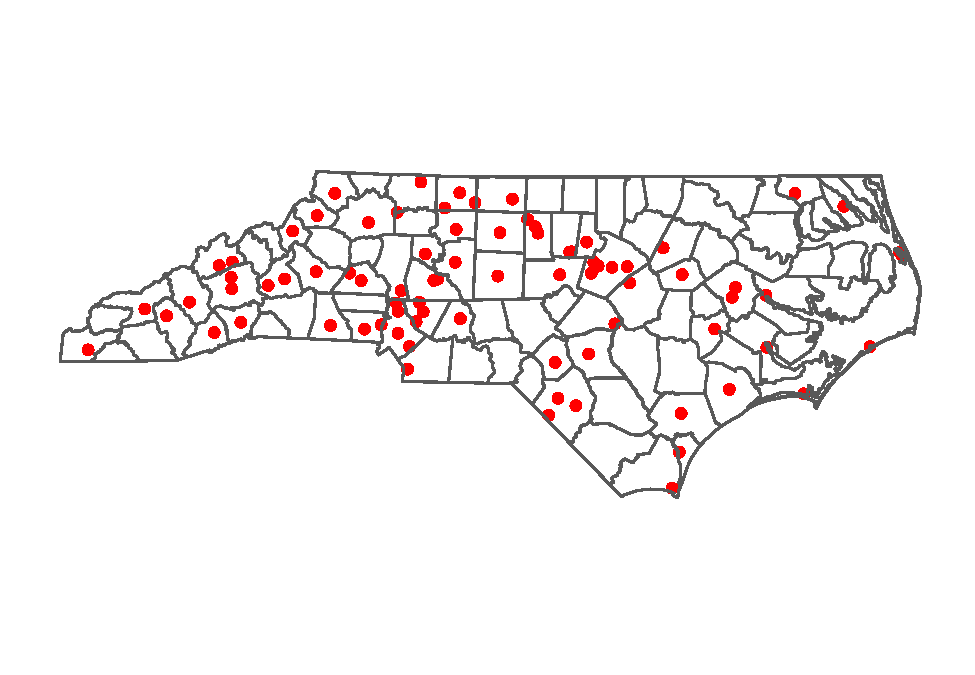
\includegraphics[width=0.32\linewidth]{asa_abstract_files/figure-latex/figures-side-2} 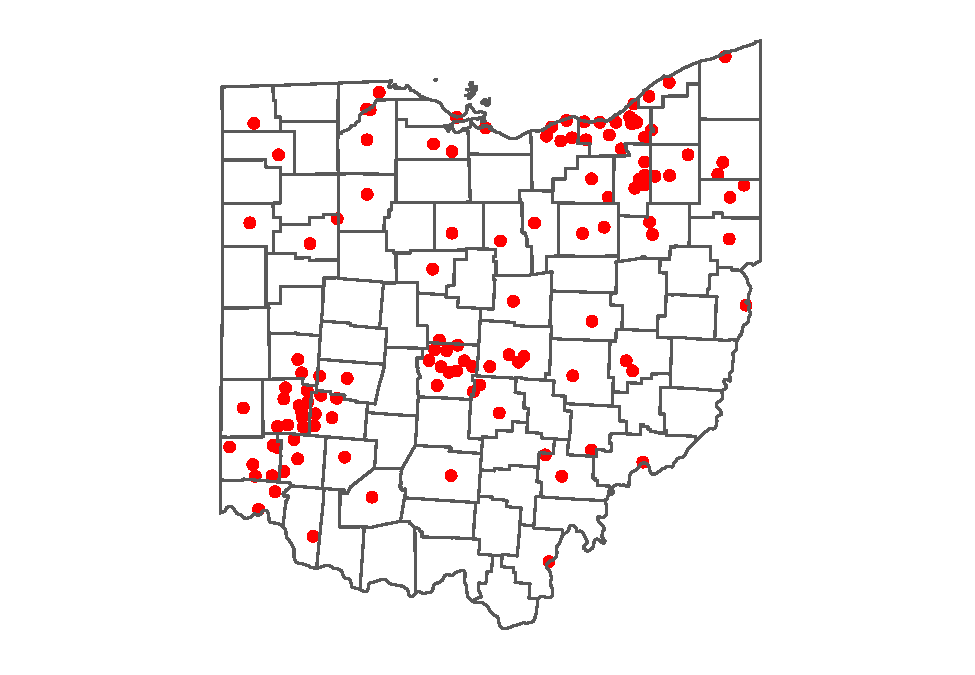
\includegraphics[width=0.32\linewidth]{asa_abstract_files/figure-latex/figures-side-3} \caption{\label{fig:map}Protest Sites, June 2020}\label{fig:figures-side}
\end{figure}

Table \ref{tab:reg} reports the results of an ordinary least squares regression, where each observation is a registered voter. The dependent variable \emph{Voted in 2020} measures whether a voter participated in the 2020 general election, and the primary independent variable \emph{Distance} measures how far the voter lived from the nearest June protest in their state. We also control for other individual and neighborhood-level characteristics, including each voter's own participation history. Robust standard errors are clustered by county.\footnote{These are currently run on random 10 percent samples, stratified by county, due to computing restraints. Eventually, full models will be run using the complete universe of voters.}

\begin{singlespace}
\input{"../temp/big_reg_formatted.tex"}
\end{singlespace}

In all three states, our preliminary models indicate that voters who lived closer to June protests actually turned out at \emph{lower} rates, even after controlling for other relevant characteristics including each voter's own vote history, population density, and county fixed effects. While the linear term is not statistically significant in the first North Carolina model, the relationship is significant in the model where the squared term is included. In both Georgia and North Carolina, turnout was about 1 percentage point lower for voters who lived within 5 miles of the closest protest than for other voters. Turnout was 2.8 percentage points lower for these voters in Ohio.

Because the magnitudes of the coefficients are not immediately obvious, we include the marginal effects plots of the linear and squared models in the Appendix.

\hypertarget{what-comes-next}{%
\subsubsection*{What Comes Next}\label{what-comes-next}}
\addcontentsline{toc}{subsubsection}{What Comes Next}

Our preliminary results indicate that the relationship between distance to protests and turnout is more complicated than we initially expected. This is perhaps true for both methodological and theoretical reasons. Methodologically, we have not yet implemented the instrumental variable approach that will allow us to more precisely estimate the causal effect of protest exposure. Further, the clustered distribution of protests evident in Figure \ref{fig:map} demonstrates a need for spatial regression techniques to fully account for spatial autocorrelation. Theoretically, it may be that protest exposure has disparate effects on different voters, and that a single estimate of exposure masks heterogeneous effects. We plan to explore these aspects in our full paper.

\newpage

\hypertarget{references}{%
\subsection*{References}\label{references}}
\addcontentsline{toc}{subsection}{References}

\hypertarget{refs}{}
\begin{cslreferences}
\leavevmode\hypertarget{ref-Bell2017}{}%
Bell, Monica C. 2017. ``Police Reform and the Dismantling of Legal Estrangement.'' \emph{The Yale Law Journal} 126 (7): 2054--2150. \url{http://www.jstor.org/stable/45222555}.

\leavevmode\hypertarget{ref-Brayne2014}{}%
Brayne, Sarah. 2014. ``Surveillance and System Avoidance: Criminal Justice Contact and Institutional Attachment.'' \emph{American Sociological Review} 79 (3): 367--91. \url{https://doi.org/10.1177/0003122414530398}.

\leavevmode\hypertarget{ref-Fillieule2013}{}%
Fillieule, Olivier. 2013. ``Political Socialization and Social Movements.'' In \emph{The Wiley-Blackwell Encyclopedia of Social and Political Movements}. American Cancer Society. \url{https://doi.org/10.1002/9780470674871.wbespm199}.

\leavevmode\hypertarget{ref-Kirk2011}{}%
Kirk, David S., and Andrew V. Papachristos. 2011. ``Cultural Mechanisms and the Persistence of Neighborhood Violence.'' \emph{American Journal of Sociology} 116 (4): 1190--1233. \url{https://doi.org/10.1086/655754}.

\leavevmode\hypertarget{ref-Leege2002}{}%
Leege, David C., Kenneth D. Wald, Brian S. Krueger, and Paul D. Mueller. 2002. \emph{The Politics of Cultural Differences: Social Change and Voter Mobilization Strategies in the Post-New Deal Period}. Princeton: Princeton University Press.

\leavevmode\hypertarget{ref-Lerman2014}{}%
Lerman, Amy E., and Vesla M. Weaver. 2014. \emph{Arresting Citizenship: The Democratic Consequences of American Crime Control}. Chicago Studies in American Politics. Chicago ; London: The University of Chicago Press.

\leavevmode\hypertarget{ref-Madestam2013}{}%
Madestam, Andreas, Daniel Shoag, Stan Veuger, and David Yanagizawa-Drott. 2013. ``Do Political Protests Matter? Evidence from the Tea Party Movement*.'' \emph{The Quarterly Journal of Economics} 128 (4): 1633--85. \url{https://doi.org/10.1093/qje/qjt021}.

\leavevmode\hypertarget{ref-McAdam1989}{}%
McAdam, Doug. 1989. ``The Biographical Consequences of Activism.'' \emph{American Sociological Review} 54 (5): 744--60. \url{https://doi.org/10.2307/2117751}.

\leavevmode\hypertarget{ref-Morris2020}{}%
Morris, Kevin. 2020. ``Neighborhoods and Felony Disenfranchisement: The Case of New York City.'' \emph{Urban Affairs Review}, May, 1078087420921522. \url{https://doi.org/10.1177/1078087420921522}.

\leavevmode\hypertarget{ref-Sherkat1997}{}%
Sherkat, Darren E., and T. Jean Blocker. 1997. ``Explaining the Political and Personal Consequences of Protest.'' \emph{Social Forces} 75 (3): 1049--70. \url{https://doi.org/10.2307/2580530}.

\leavevmode\hypertarget{ref-Snow1986}{}%
Snow, David A., E. Burke Rochford, Steven K. Worden, and Robert D. Benford. 1986. ``Frame Alignment Processes, Micromobilization, and Movement Participation.'' \emph{American Sociological Review} 51 (4): 464--81. \url{https://doi.org/10.2307/2095581}.

\leavevmode\hypertarget{ref-Walker2014}{}%
Walker, Hannah L. 2014. ``Extending the Effects of the Carceral State: Proximal Contact, Political Participation, and Race.'' \emph{Political Research Quarterly}, July. \url{https://doi.org/10.1177/1065912914542522}.

\leavevmode\hypertarget{ref-Walker2020}{}%
---------. 2020. ``Targeted: The Mobilizing Effect of Perceptions of Unfair Policing Practices.'' \emph{The Journal of Politics} 82 (1): 119--34. \url{https://doi.org/10.1086/705684}.

\leavevmode\hypertarget{ref-White2019}{}%
White, Ariel. 2019. ``Family Matters? Voting Behavior in Households with Criminal Justice Contact.'' \emph{American Political Science Review} 113 (2): 607--13. \url{https://doi.org/10.1017/S0003055418000862}.

\leavevmode\hypertarget{ref-Winders1999}{}%
Winders, Bill. 1999. ``The Roller Coaster of Class Conflict: Class Segments, Mass Mobilization, and Voter Turnout in the U.S., 1840-1996.'' \emph{Social Forces} 77 (3): 833--62. \url{https://doi.org/10.2307/3005963}.
\end{cslreferences}

\newpage
\pagenumbering{gobble}
\pagenumbering{arabic}

\hypertarget{appendix}{%
\subsection*{Appendix}\label{appendix}}
\addcontentsline{toc}{subsection}{Appendix}

\begin{figure}[H]

{\centering 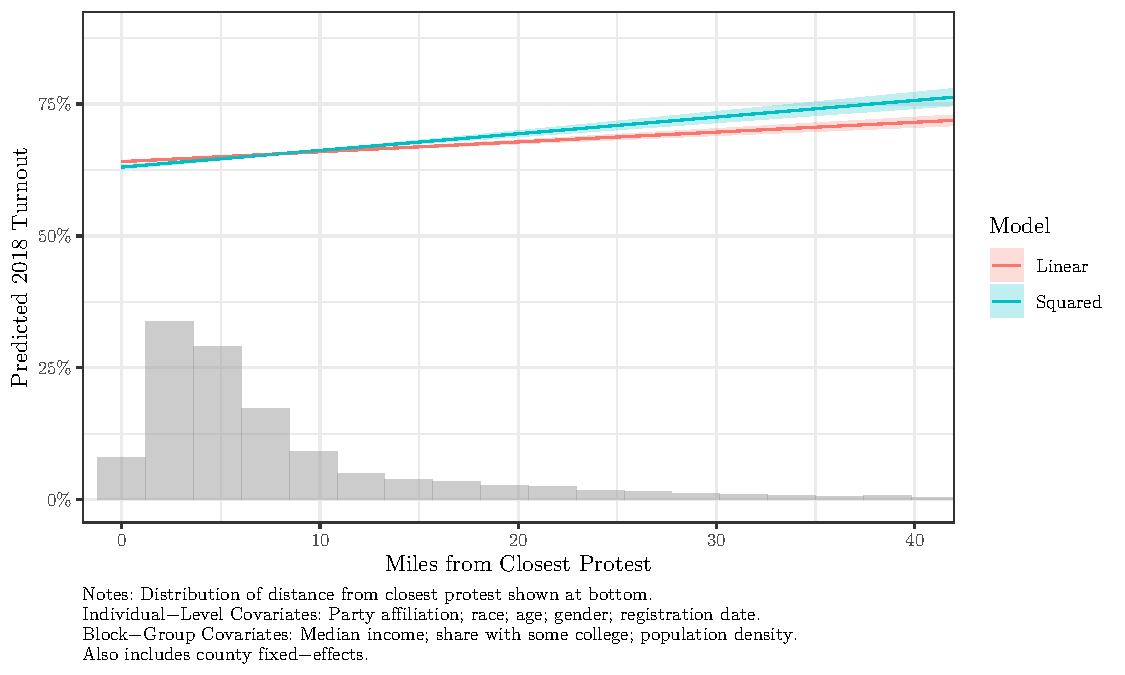
\includegraphics{asa_abstract_files/figure-latex/ga-plot-1} 

}

\caption{\label{fig:ga}Maringal Effect of Distance from Closest Protest on Predicted Turnout, GA}\label{fig:ga-plot}
\end{figure}

\begin{figure}[H]

{\centering 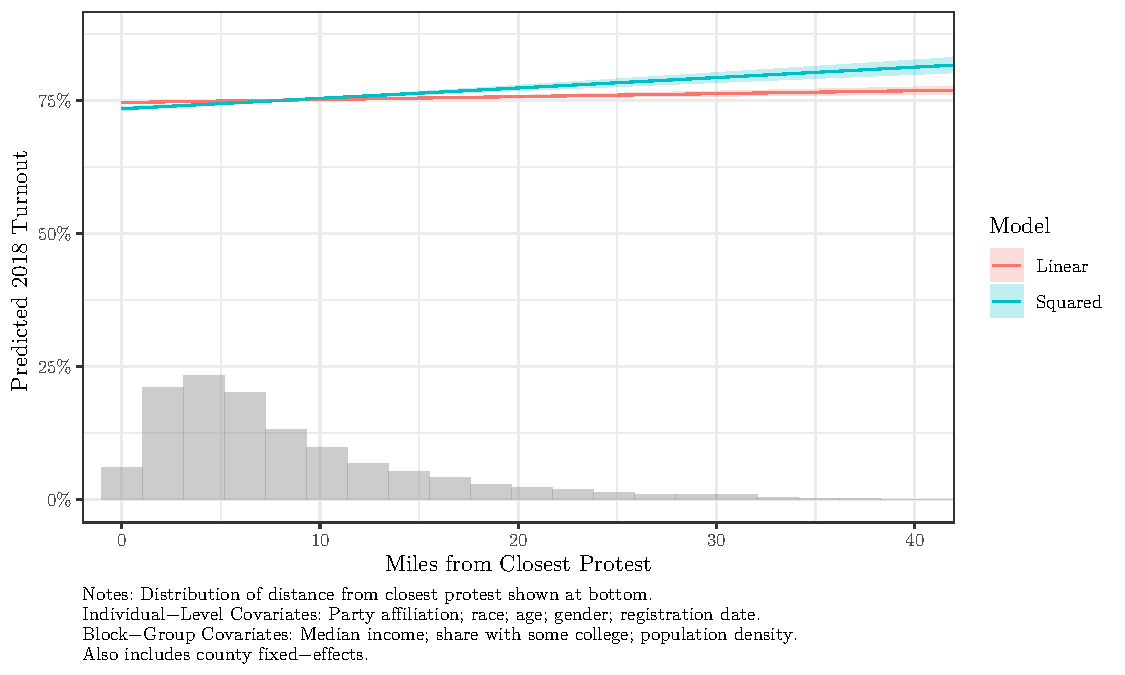
\includegraphics{asa_abstract_files/figure-latex/nc-plot-1} 

}

\caption{\label{fig:ga}Maringal Effect of Distance from Closest Protest on Predicted Turnout, NC}\label{fig:nc-plot}
\end{figure}

\begin{figure}[H]

{\centering 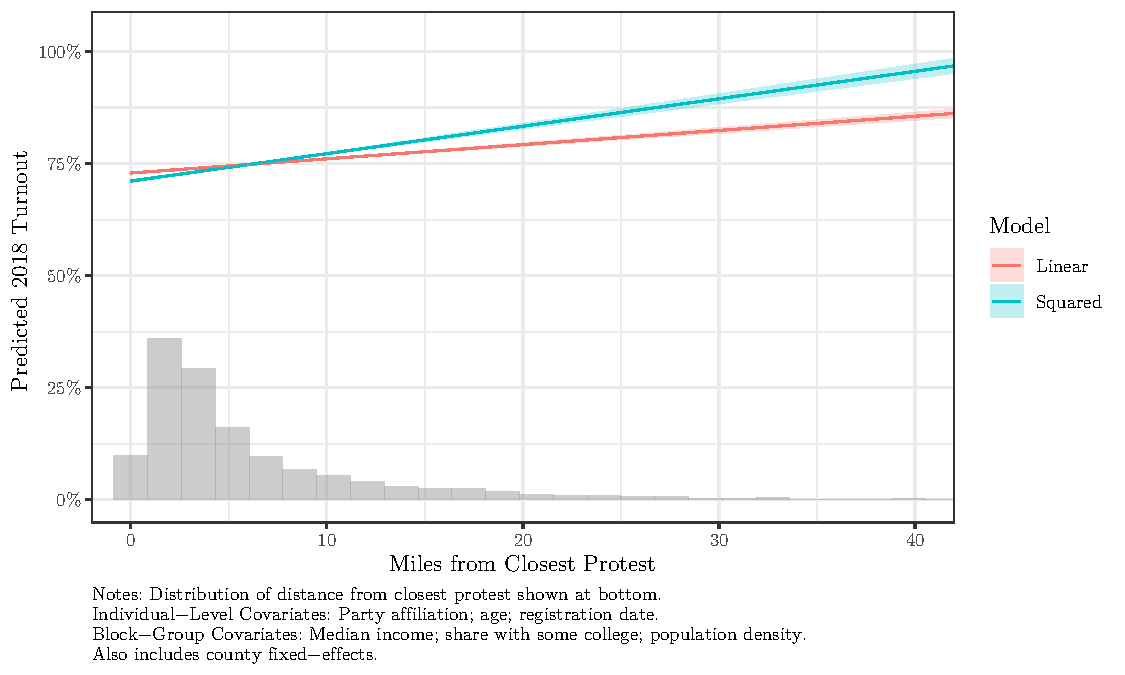
\includegraphics{asa_abstract_files/figure-latex/oh-plot-1} 

}

\caption{\label{fig:ga}Maringal Effect of Distance from Closest Protest on Predicted Turnout, OH}\label{fig:oh-plot}
\end{figure}

\end{document}
